\documentclass[1p]{elsarticle_modified}
%\bibliographystyle{elsarticle-num}

%\usepackage[colorlinks]{hyperref}
%\usepackage{abbrmath_seonhwa} %\Abb, \Ascr, \Acal ,\Abf, \Afrak
\usepackage{amsfonts}
\usepackage{amssymb}
\usepackage{amsmath}
\usepackage{amsthm}
\usepackage{scalefnt}
\usepackage{amsbsy}
\usepackage{kotex}
\usepackage{caption}
\usepackage{subfig}
\usepackage{color}
\usepackage{graphicx}
\usepackage{xcolor} %% white, black, red, green, blue, cyan, magenta, yellow
\usepackage{float}
\usepackage{setspace}
\usepackage{hyperref}

\usepackage{tikz}
\usetikzlibrary{arrows}

\usepackage{multirow}
\usepackage{array} % fixed length table
\usepackage{hhline}

%%%%%%%%%%%%%%%%%%%%%
\makeatletter
\renewcommand*\env@matrix[1][\arraystretch]{%
	\edef\arraystretch{#1}%
	\hskip -\arraycolsep
	\let\@ifnextchar\new@ifnextchar
	\array{*\c@MaxMatrixCols c}}
\makeatother %https://tex.stackexchange.com/questions/14071/how-can-i-increase-the-line-spacing-in-a-matrix
%%%%%%%%%%%%%%%

\usepackage[normalem]{ulem}

\newcommand{\msout}[1]{\ifmmode\text{\sout{\ensuremath{#1}}}\else\sout{#1}\fi}
%SOURCE: \msout is \stkout macro in https://tex.stackexchange.com/questions/20609/strikeout-in-math-mode

\newcommand{\cancel}[1]{
	\ifmmode
	{\color{red}\msout{#1}}
	\else
	{\color{red}\sout{#1}}
	\fi
}

\newcommand{\add}[1]{
	{\color{blue}\uwave{#1}}
}

\newcommand{\replace}[2]{
	\ifmmode
	{\color{red}\msout{#1}}{\color{blue}\uwave{#2}}
	\else
	{\color{red}\sout{#1}}{\color{blue}\uwave{#2}}
	\fi
}

\newcommand{\Sol}{\mathcal{S}} %segment
\newcommand{\D}{D} %diagram
\newcommand{\A}{\mathcal{A}} %arc


%%%%%%%%%%%%%%%%%%%%%%%%%%%%%5 test

\def\sl{\operatorname{\textup{SL}}(2,\Cbb)}
\def\psl{\operatorname{\textup{PSL}}(2,\Cbb)}
\def\quan{\mkern 1mu \triangleright \mkern 1mu}

\theoremstyle{definition}
\newtheorem{thm}{Theorem}[section]
\newtheorem{prop}[thm]{Proposition}
\newtheorem{lem}[thm]{Lemma}
\newtheorem{ques}[thm]{Question}
\newtheorem{cor}[thm]{Corollary}
\newtheorem{defn}[thm]{Definition}
\newtheorem{exam}[thm]{Example}
\newtheorem{rmk}[thm]{Remark}
\newtheorem{alg}[thm]{Algorithm}

\newcommand{\I}{\sqrt{-1}}
\begin{document}

%\begin{frontmatter}
%
%\title{Boundary parabolic representations of knots up to 8 crossings}
%
%%% Group authors per affiliation:
%\author{Yunhi Cho} 
%\address{Department of Mathematics, University of Seoul, Seoul, Korea}
%\ead{yhcho@uos.ac.kr}
%
%
%\author{Seonhwa Kim} %\fnref{s_kim}}
%\address{Center for Geometry and Physics, Institute for Basic Science, Pohang, 37673, Korea}
%\ead{ryeona17@ibs.re.kr}
%
%\author{Hyuk Kim}
%\address{Department of Mathematical Sciences, Seoul National University, Seoul 08826, Korea}
%\ead{hyukkim@snu.ac.kr}
%
%\author{Seokbeom Yoon}
%\address{Department of Mathematical Sciences, Seoul National University, Seoul, 08826,  Korea}
%\ead{sbyoon15@snu.ac.kr}
%
%\begin{abstract}
%We find all boundary parabolic representation of knots up to 8 crossings.
%
%\end{abstract}
%\begin{keyword}
%    \MSC[2010] 57M25 
%\end{keyword}
%
%\end{frontmatter}

%\linenumbers
%\tableofcontents
%
\newcommand\colored[1]{\textcolor{white}{\rule[-0.35ex]{0.8em}{1.4ex}}\kern-0.8em\color{red} #1}%
%\newcommand\colored[1]{\textcolor{white}{ #1}\kern-2.17ex	\textcolor{white}{ #1}\kern-1.81ex	\textcolor{white}{ #1}\kern-2.15ex\color{red}#1	}

{\Large $\underline{11a_{156}~(K11a_{156})}$}

\setlength{\tabcolsep}{10pt}
\renewcommand{\arraystretch}{1.6}
\vspace{1cm}\begin{tabular}{m{100pt}>{\centering\arraybackslash}m{274pt}}
\multirow{5}{120pt}{
	\centering
	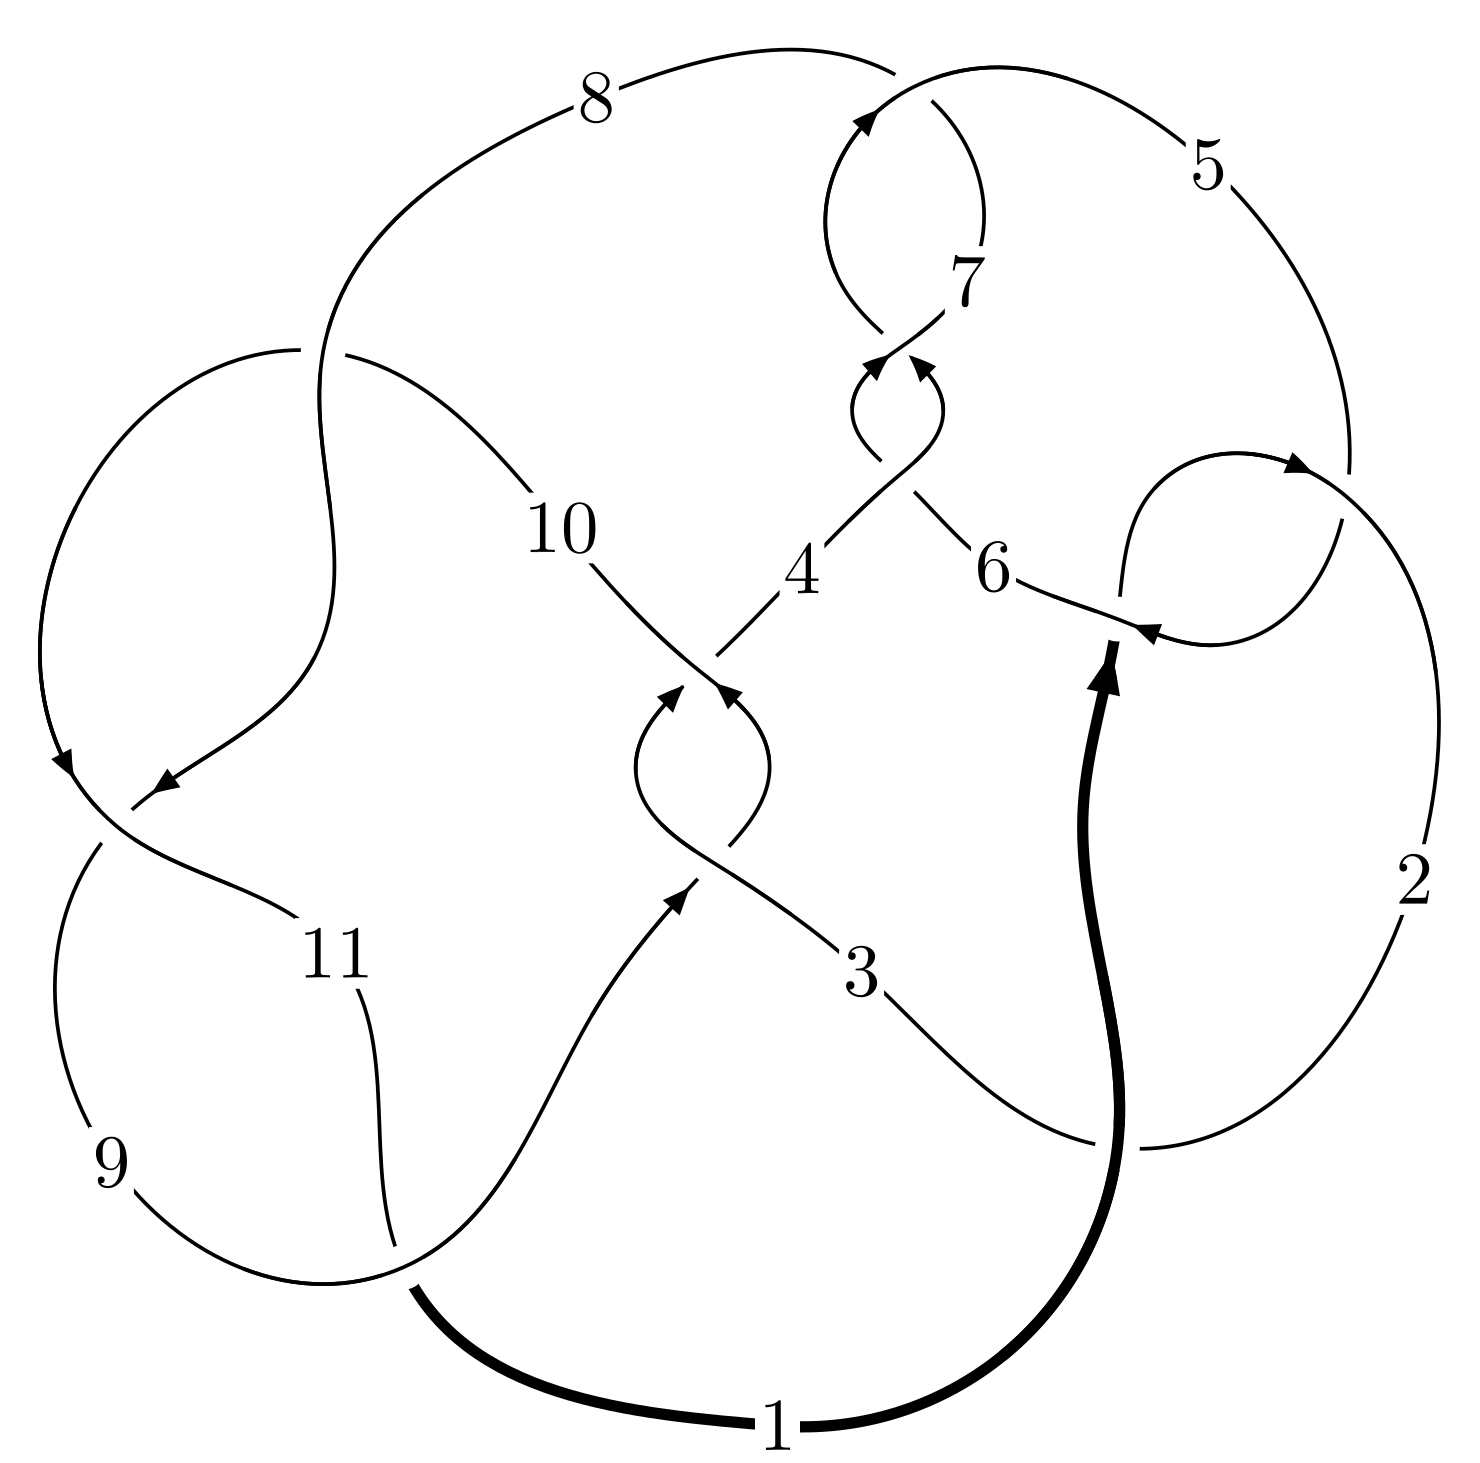
\includegraphics[width=112pt]{../../../GIT/diagram.site/Diagrams/png/405_11a_156.png}\\
\ \ \ A knot diagram\footnotemark}&
\allowdisplaybreaks
\textbf{Linearized knot diagam} \\
\cline{2-2}
 &
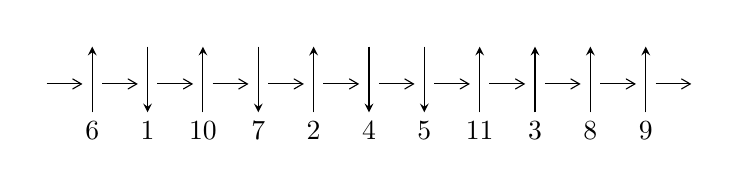
\begin{tikzpicture}[x=20pt, y=17pt]
	% nodes
	\node (C0) at (0, 0) {};
	\node (C1) at (1, 0) {};
	\node (C1U) at (1, +1) {};
	\node (C1D) at (1, -1) {6};

	\node (C2) at (2, 0) {};
	\node (C2U) at (2, +1) {};
	\node (C2D) at (2, -1) {1};

	\node (C3) at (3, 0) {};
	\node (C3U) at (3, +1) {};
	\node (C3D) at (3, -1) {10};

	\node (C4) at (4, 0) {};
	\node (C4U) at (4, +1) {};
	\node (C4D) at (4, -1) {7};

	\node (C5) at (5, 0) {};
	\node (C5U) at (5, +1) {};
	\node (C5D) at (5, -1) {2};

	\node (C6) at (6, 0) {};
	\node (C6U) at (6, +1) {};
	\node (C6D) at (6, -1) {4};

	\node (C7) at (7, 0) {};
	\node (C7U) at (7, +1) {};
	\node (C7D) at (7, -1) {5};

	\node (C8) at (8, 0) {};
	\node (C8U) at (8, +1) {};
	\node (C8D) at (8, -1) {11};

	\node (C9) at (9, 0) {};
	\node (C9U) at (9, +1) {};
	\node (C9D) at (9, -1) {3};

	\node (C10) at (10, 0) {};
	\node (C10U) at (10, +1) {};
	\node (C10D) at (10, -1) {8};

	\node (C11) at (11, 0) {};
	\node (C11U) at (11, +1) {};
	\node (C11D) at (11, -1) {9};
	\node (C12) at (12, 0) {};

	% arrows
	\draw[->,>={angle 60}]
	(C0) edge (C1) (C1) edge (C2) (C2) edge (C3) (C3) edge (C4) (C4) edge (C5) (C5) edge (C6) (C6) edge (C7) (C7) edge (C8) (C8) edge (C9) (C9) edge (C10) (C10) edge (C11) (C11) edge (C12) ;	\draw[->,>=stealth]
	(C1D) edge (C1U) (C2U) edge (C2D) (C3D) edge (C3U) (C4U) edge (C4D) (C5D) edge (C5U) (C6U) edge (C6D) (C7U) edge (C7D) (C8D) edge (C8U) (C9D) edge (C9U) (C10D) edge (C10U) (C11D) edge (C11U) ;
	\end{tikzpicture} \\
\hhline{~~} \\& 
\textbf{Solving Sequence} \\ \cline{2-2} 
 &
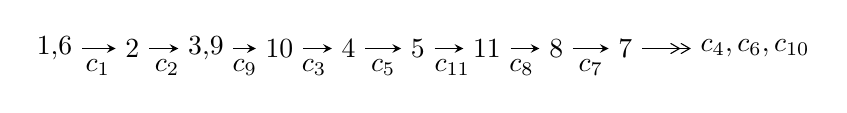
\begin{tikzpicture}[x=25pt, y=7pt]
	% node
	\node (A0) at (-1/8, 0) {1,6};
	\node (A1) at (1, 0) {2};
	\node (A2) at (33/16, 0) {3,9};
	\node (A3) at (25/8, 0) {10};
	\node (A4) at (33/8, 0) {4};
	\node (A5) at (41/8, 0) {5};
	\node (A6) at (49/8, 0) {11};
	\node (A7) at (57/8, 0) {8};
	\node (A8) at (65/8, 0) {7};
	\node (C1) at (1/2, -1) {$c_{1}$};
	\node (C2) at (3/2, -1) {$c_{2}$};
	\node (C3) at (21/8, -1) {$c_{9}$};
	\node (C4) at (29/8, -1) {$c_{3}$};
	\node (C5) at (37/8, -1) {$c_{5}$};
	\node (C6) at (45/8, -1) {$c_{11}$};
	\node (C7) at (53/8, -1) {$c_{8}$};
	\node (C8) at (61/8, -1) {$c_{7}$};
	\node (A9) at (10, 0) {$c_{4},c_{6},c_{10}$};

	% edge
	\draw[->,>=stealth]	
	(A0) edge (A1) (A1) edge (A2) (A2) edge (A3) (A3) edge (A4) (A4) edge (A5) (A5) edge (A6) (A6) edge (A7) (A7) edge (A8) ;
	\draw[->>,>={angle 60}]	
	(A8) edge (A9);
\end{tikzpicture} \\ 

\end{tabular} \\

\footnotetext{
The image of knot diagram is generated by the software ``\textbf{Draw programme}" developed by Andrew Bartholomew(\url{http://www.layer8.co.uk/maths/draw/index.htm\#Running-draw}), where we modified some parts for our purpose(\url{https://github.com/CATsTAILs/LinksPainter}).
}\phantom \\ \newline 
\centering \textbf{Ideals for irreducible components\footnotemark of $X_{\text{par}}$} 
 
\begin{align*}
I^u_{1}&=\langle 
1.35866\times10^{48} u^{51}-1.57104\times10^{48} u^{50}+\cdots+3.08851\times10^{48} b+4.21202\times10^{48},\\
\phantom{I^u_{1}}&\phantom{= \langle  }-1.52481\times10^{49} u^{51}+2.17161\times10^{49} u^{50}+\cdots+6.17703\times10^{48} a-1.53352\times10^{50},\\
\phantom{I^u_{1}}&\phantom{= \langle  }u^{52}-2 u^{51}+\cdots+28 u-4\rangle \\
I^u_{2}&=\langle 
b-1,\;u^4+u^2+a+u+1,\;u^5- u^4+2 u^3- u^2+u-1\rangle \\
\\
I^v_{1}&=\langle 
a,\;b- v+2,\;v^2-3 v+1\rangle \\
\end{align*}
\raggedright * 3 irreducible components of $\dim_{\mathbb{C}}=0$, with total 59 representations.\\
\footnotetext{All coefficients of polynomials are rational numbers. But the coefficients are sometimes approximated in decimal forms when there is not enough margin.}
\newpage
\renewcommand{\arraystretch}{1}
\centering \section*{I. $I^u_{1}= \langle 1.36\times10^{48} u^{51}-1.57\times10^{48} u^{50}+\cdots+3.09\times10^{48} b+4.21\times10^{48},\;-1.52\times10^{49} u^{51}+2.17\times10^{49} u^{50}+\cdots+6.18\times10^{48} a-1.53\times10^{50},\;u^{52}-2 u^{51}+\cdots+28 u-4 \rangle$}
\flushleft \textbf{(i) Arc colorings}\\
\begin{tabular}{m{7pt} m{180pt} m{7pt} m{180pt} }
\flushright $a_{1}=$&$\begin{pmatrix}1\\0\end{pmatrix}$ \\
\flushright $a_{6}=$&$\begin{pmatrix}0\\u\end{pmatrix}$ \\
\flushright $a_{2}=$&$\begin{pmatrix}1\\- u^2\end{pmatrix}$ \\
\flushright $a_{3}=$&$\begin{pmatrix}u^2+1\\- u^2\end{pmatrix}$ \\
\flushright $a_{9}=$&$\begin{pmatrix}2.46852 u^{51}-3.51562 u^{50}+\cdots-104.235 u+24.8262\\-0.439906 u^{51}+0.508672 u^{50}+\cdots+10.8322 u-1.36377\end{pmatrix}$ \\
\flushright $a_{10}=$&$\begin{pmatrix}2.84368 u^{51}-4.05858 u^{50}+\cdots-117.062 u+28.1494\\-0.556181 u^{51}+0.655346 u^{50}+\cdots+13.1982 u-1.84971\end{pmatrix}$ \\
\flushright $a_{4}=$&$\begin{pmatrix}0.770801 u^{51}-0.938728 u^{50}+\cdots-26.6783 u+6.61543\\-0.576000 u^{51}+0.735448 u^{50}+\cdots+12.0720 u-2.35162\end{pmatrix}$ \\
\flushright $a_{5}=$&$\begin{pmatrix}- u\\u^3+u\end{pmatrix}$ \\
\flushright $a_{11}=$&$\begin{pmatrix}1.96321 u^{51}-3.05211 u^{50}+\cdots-93.6559 u+23.1027\\0.0420101 u^{51}+0.0759082 u^{50}+\cdots+7.19593 u-1.40746\end{pmatrix}$ \\
\flushright $a_{8}=$&$\begin{pmatrix}0.194801 u^{51}-0.203280 u^{50}+\cdots-14.6063 u+4.26381\\0.243803 u^{51}-0.393136 u^{50}+\cdots-7.63417 u+1.60634\end{pmatrix}$ \\
\flushright $a_{7}=$&$\begin{pmatrix}0.685271 u^{51}-0.920162 u^{50}+\cdots-28.4036 u+6.67530\\-0.226462 u^{51}+0.539033 u^{50}+\cdots+11.5948 u-1.86138\end{pmatrix}$\\ \flushright $a_{7}=$&$\begin{pmatrix}0.685271 u^{51}-0.920162 u^{50}+\cdots-28.4036 u+6.67530\\-0.226462 u^{51}+0.539033 u^{50}+\cdots+11.5948 u-1.86138\end{pmatrix}$\\&\end{tabular}
\flushleft \textbf{(ii) Obstruction class $= -1$}\\~\\
\flushleft \textbf{(iii) Cusp Shapes $= -6.29255 u^{51}+9.41983 u^{50}+\cdots+269.288 u-54.6478$}\\~\\
\newpage\renewcommand{\arraystretch}{1}
\flushleft \textbf{(iv) u-Polynomials at the component}\newline \\
\begin{tabular}{m{50pt}|m{274pt}}
Crossings & \hspace{64pt}u-Polynomials at each crossing \\
\hline $$\begin{aligned}c_{1},c_{5}\end{aligned}$$&$\begin{aligned}
&u^{52}-2 u^{51}+\cdots+28 u-4
\end{aligned}$\\
\hline $$\begin{aligned}c_{2}\end{aligned}$$&$\begin{aligned}
&u^{52}+18 u^{51}+\cdots-72 u+16
\end{aligned}$\\
\hline $$\begin{aligned}c_{3},c_{9}\end{aligned}$$&$\begin{aligned}
&u^{52}-2 u^{51}+\cdots+64 u-32
\end{aligned}$\\
\hline $$\begin{aligned}c_{4},c_{6},c_{7}\end{aligned}$$&$\begin{aligned}
&u^{52}-4 u^{51}+\cdots-4 u+1
\end{aligned}$\\
\hline $$\begin{aligned}c_{8},c_{10},c_{11}\end{aligned}$$&$\begin{aligned}
&u^{52}+7 u^{51}+\cdots+3 u+1
\end{aligned}$\\
\hline
\end{tabular}\\~\\
\newpage\renewcommand{\arraystretch}{1}
\flushleft \textbf{(v) Riley Polynomials at the component}\newline \\
\begin{tabular}{m{50pt}|m{274pt}}
Crossings & \hspace{64pt}Riley Polynomials at each crossing \\
\hline $$\begin{aligned}c_{1},c_{5}\end{aligned}$$&$\begin{aligned}
&y^{52}+18 y^{51}+\cdots-72 y+16
\end{aligned}$\\
\hline $$\begin{aligned}c_{2}\end{aligned}$$&$\begin{aligned}
&y^{52}+30 y^{51}+\cdots-41760 y+256
\end{aligned}$\\
\hline $$\begin{aligned}c_{3},c_{9}\end{aligned}$$&$\begin{aligned}
&y^{52}-36 y^{51}+\cdots-10752 y+1024
\end{aligned}$\\
\hline $$\begin{aligned}c_{4},c_{6},c_{7}\end{aligned}$$&$\begin{aligned}
&y^{52}-44 y^{51}+\cdots-116 y+1
\end{aligned}$\\
\hline $$\begin{aligned}c_{8},c_{10},c_{11}\end{aligned}$$&$\begin{aligned}
&y^{52}-53 y^{51}+\cdots+13 y+1
\end{aligned}$\\
\hline
\end{tabular}\\~\\
\newpage\flushleft \textbf{(vi) Complex Volumes and Cusp Shapes}
$$\begin{array}{c|c|c}  
\text{Solutions to }I^u_{1}& \I (\text{vol} + \sqrt{-1}CS) & \text{Cusp shape}\\
 \hline 
\begin{aligned}
u &= \phantom{-}0.075327 + 1.008500 I \\
a &= -1.022790 + 0.774917 I \\
b &= \phantom{-}1.190360 + 0.416488 I\end{aligned}
 & -3.66540 + 1.40599 I & -0.611498 - 0.934044 I \\ \hline\begin{aligned}
u &= \phantom{-}0.075327 - 1.008500 I \\
a &= -1.022790 - 0.774917 I \\
b &= \phantom{-}1.190360 - 0.416488 I\end{aligned}
 & -3.66540 - 1.40599 I & -0.611498 + 0.934044 I \\ \hline\begin{aligned}
u &= \phantom{-}0.613736 + 0.753703 I \\
a &= -1.05975 + 1.15611 I \\
b &= \phantom{-}0.527758 + 0.653505 I\end{aligned}
 & \phantom{-}0.194027 + 1.037730 I & \phantom{-}3.66549 - 3.70521 I \\ \hline\begin{aligned}
u &= \phantom{-}0.613736 - 0.753703 I \\
a &= -1.05975 - 1.15611 I \\
b &= \phantom{-}0.527758 - 0.653505 I\end{aligned}
 & \phantom{-}0.194027 - 1.037730 I & \phantom{-}3.66549 + 3.70521 I \\ \hline\begin{aligned}
u &= -0.772235 + 0.690068 I \\
a &= -2.53064 - 1.27133 I \\
b &= \phantom{-}1.378930 + 0.036041 I\end{aligned}
 & \phantom{-}2.12355 + 1.28202 I & \phantom{-}4.52218 - 0.37137 I \\ \hline\begin{aligned}
u &= -0.772235 - 0.690068 I \\
a &= -2.53064 + 1.27133 I \\
b &= \phantom{-}1.378930 - 0.036041 I\end{aligned}
 & \phantom{-}2.12355 - 1.28202 I & \phantom{-}4.52218 + 0.37137 I \\ \hline\begin{aligned}
u &= \phantom{-}0.455162 + 0.835894 I \\
a &= \phantom{-}0.863304 - 0.362503 I \\
b &= -0.263353 - 0.185170 I\end{aligned}
 & -0.04711 + 1.88095 I & -0.11775 - 4.20113 I \\ \hline\begin{aligned}
u &= \phantom{-}0.455162 - 0.835894 I \\
a &= \phantom{-}0.863304 + 0.362503 I \\
b &= -0.263353 + 0.185170 I\end{aligned}
 & -0.04711 - 1.88095 I & -0.11775 + 4.20113 I \\ \hline\begin{aligned}
u &= -0.729350 + 0.773257 I \\
a &= -0.108923 - 0.214082 I \\
b &= \phantom{-}0.639530 + 0.722525 I\end{aligned}
 & \phantom{-}3.67881 - 0.13440 I & \phantom{-}8.39486 + 0. I\phantom{ +0.000000I} \\ \hline\begin{aligned}
u &= -0.729350 - 0.773257 I \\
a &= -0.108923 + 0.214082 I \\
b &= \phantom{-}0.639530 - 0.722525 I\end{aligned}
 & \phantom{-}3.67881 + 0.13440 I & \phantom{-}8.39486 + 0. I\phantom{ +0.000000I}\\
 \hline 
 \end{array}$$\newpage$$\begin{array}{c|c|c}  
\text{Solutions to }I^u_{1}& \I (\text{vol} + \sqrt{-1}CS) & \text{Cusp shape}\\
 \hline 
\begin{aligned}
u &= \phantom{-}0.886765 + 0.619894 I \\
a &= \phantom{-}0.076581 + 0.354456 I \\
b &= \phantom{-}0.461865 - 0.742040 I\end{aligned}
 & -0.14154 - 3.59160 I & \phantom{-}3.36417 + 4.10455 I \\ \hline\begin{aligned}
u &= \phantom{-}0.886765 - 0.619894 I \\
a &= \phantom{-}0.076581 - 0.354456 I \\
b &= \phantom{-}0.461865 + 0.742040 I\end{aligned}
 & -0.14154 + 3.59160 I & \phantom{-}3.36417 - 4.10455 I \\ \hline\begin{aligned}
u &= \phantom{-}0.619534 + 0.655112 I \\
a &= \phantom{-}1.82077 - 0.13795 I \\
b &= -1.62890 + 0.13929 I\end{aligned}
 & \phantom{-}7.94427 + 0.70276 I & \phantom{-}6.08078 - 4.95980 I \\ \hline\begin{aligned}
u &= \phantom{-}0.619534 - 0.655112 I \\
a &= \phantom{-}1.82077 + 0.13795 I \\
b &= -1.62890 - 0.13929 I\end{aligned}
 & \phantom{-}7.94427 - 0.70276 I & \phantom{-}6.08078 + 4.95980 I \\ \hline\begin{aligned}
u &= -0.906927 + 0.670128 I \\
a &= \phantom{-}1.75190 + 0.21463 I \\
b &= -1.55769 - 0.21556 I\end{aligned}
 & \phantom{-}10.93850 + 3.24486 I & \phantom{-}10.33648 - 1.31467 I \\ \hline\begin{aligned}
u &= -0.906927 - 0.670128 I \\
a &= \phantom{-}1.75190 - 0.21463 I \\
b &= -1.55769 + 0.21556 I\end{aligned}
 & \phantom{-}10.93850 - 3.24486 I & \phantom{-}10.33648 + 1.31467 I \\ \hline\begin{aligned}
u &= \phantom{-}0.732657 + 0.866743 I \\
a &= -2.26559 + 1.11526 I \\
b &= \phantom{-}1.43928 + 0.05940 I\end{aligned}
 & \phantom{-}5.55338 + 2.78570 I & \phantom{-}8.09999 - 3.02309 I \\ \hline\begin{aligned}
u &= \phantom{-}0.732657 - 0.866743 I \\
a &= -2.26559 - 1.11526 I \\
b &= \phantom{-}1.43928 - 0.05940 I\end{aligned}
 & \phantom{-}5.55338 - 2.78570 I & \phantom{-}8.09999 + 3.02309 I \\ \hline\begin{aligned}
u &= \phantom{-}0.635920 + 0.950705 I \\
a &= -0.338552 + 0.157448 I \\
b &= \phantom{-}0.792480 - 0.758107 I\end{aligned}
 & -0.43994 + 3.90031 I & \phantom{-}3.00000 - 3.18847 I \\ \hline\begin{aligned}
u &= \phantom{-}0.635920 - 0.950705 I \\
a &= -0.338552 - 0.157448 I \\
b &= \phantom{-}0.792480 + 0.758107 I\end{aligned}
 & -0.43994 - 3.90031 I & \phantom{-}3.00000 + 3.18847 I\\
 \hline 
 \end{array}$$\newpage$$\begin{array}{c|c|c}  
\text{Solutions to }I^u_{1}& \I (\text{vol} + \sqrt{-1}CS) & \text{Cusp shape}\\
 \hline 
\begin{aligned}
u &= \phantom{-}0.134179 + 1.161340 I \\
a &= -0.384531 - 0.483430 I \\
b &= -1.389650 - 0.050928 I\end{aligned}
 & \phantom{-}3.59908 + 2.53417 I & \phantom{-}6.05449 - 3.57963 I \\ \hline\begin{aligned}
u &= \phantom{-}0.134179 - 1.161340 I \\
a &= -0.384531 + 0.483430 I \\
b &= -1.389650 + 0.050928 I\end{aligned}
 & \phantom{-}3.59908 - 2.53417 I & \phantom{-}6.05449 + 3.57963 I \\ \hline\begin{aligned}
u &= -0.699619 + 0.940497 I \\
a &= -0.928509 - 0.600285 I \\
b &= \phantom{-}0.486038 - 0.816981 I\end{aligned}
 & \phantom{-}3.16600 - 5.32735 I & \phantom{-0.000000 -}0. + 6.25644 I \\ \hline\begin{aligned}
u &= -0.699619 - 0.940497 I \\
a &= -0.928509 + 0.600285 I \\
b &= \phantom{-}0.486038 + 0.816981 I\end{aligned}
 & \phantom{-}3.16600 + 5.32735 I & \phantom{-0.000000 } 0. - 6.25644 I \\ \hline\begin{aligned}
u &= -0.155548 + 1.164430 I \\
a &= \phantom{-}0.234739 - 0.432223 I \\
b &= \phantom{-}0.000043 - 0.701161 I\end{aligned}
 & -7.29497 - 2.64942 I & -4.44338 + 3.34527 I \\ \hline\begin{aligned}
u &= -0.155548 - 1.164430 I \\
a &= \phantom{-}0.234739 + 0.432223 I \\
b &= \phantom{-}0.000043 + 0.701161 I\end{aligned}
 & -7.29497 + 2.64942 I & -4.44338 - 3.34527 I \\ \hline\begin{aligned}
u &= -0.785903 + 0.215104 I \\
a &= \phantom{-}0.746081 + 0.304165 I \\
b &= -0.093921 - 0.253947 I\end{aligned}
 & -2.53454 + 0.36656 I & -2.03786 + 0.85265 I \\ \hline\begin{aligned}
u &= -0.785903 - 0.215104 I \\
a &= \phantom{-}0.746081 - 0.304165 I \\
b &= -0.093921 + 0.253947 I\end{aligned}
 & -2.53454 - 0.36656 I & -2.03786 - 0.85265 I \\ \hline\begin{aligned}
u &= -1.19620\phantom{ +0.000000I} \\
a &= \phantom{-}1.56251\phantom{ +0.000000I} \\
b &= -1.37476\phantom{ +0.000000I}\end{aligned}
 & \phantom{-}1.56846\phantom{ +0.000000I} & \phantom{-}5.85290\phantom{ +0.000000I} \\ \hline\begin{aligned}
u &= \phantom{-}0.638094 + 1.019660 I \\
a &= \phantom{-}1.08345 - 1.78360 I \\
b &= -1.50936 - 0.23396 I\end{aligned}
 & \phantom{-}6.79512 + 4.31192 I & \phantom{-0.000000 } 0\\
 \hline 
 \end{array}$$\newpage$$\begin{array}{c|c|c}  
\text{Solutions to }I^u_{1}& \I (\text{vol} + \sqrt{-1}CS) & \text{Cusp shape}\\
 \hline 
\begin{aligned}
u &= \phantom{-}0.638094 - 1.019660 I \\
a &= \phantom{-}1.08345 + 1.78360 I \\
b &= -1.50936 + 0.23396 I\end{aligned}
 & \phantom{-}6.79512 - 4.31192 I & \phantom{-0.000000 } 0 \\ \hline\begin{aligned}
u &= \phantom{-}0.056951 + 0.784785 I \\
a &= \phantom{-}0.767881 + 0.964864 I \\
b &= \phantom{-}0.115114 + 0.367824 I\end{aligned}
 & -1.14630 + 1.33765 I & -2.67722 - 5.83204 I \\ \hline\begin{aligned}
u &= \phantom{-}0.056951 - 0.784785 I \\
a &= \phantom{-}0.767881 - 0.964864 I \\
b &= \phantom{-}0.115114 - 0.367824 I\end{aligned}
 & -1.14630 - 1.33765 I & -2.67722 + 5.83204 I \\ \hline\begin{aligned}
u &= -0.702251 + 0.998907 I \\
a &= -2.13606 - 0.96284 I \\
b &= \phantom{-}1.48399 - 0.13222 I\end{aligned}
 & \phantom{-}1.19040 - 6.87281 I & \phantom{-0.000000 } 0 \\ \hline\begin{aligned}
u &= -0.702251 - 0.998907 I \\
a &= -2.13606 + 0.96284 I \\
b &= \phantom{-}1.48399 + 0.13222 I\end{aligned}
 & \phantom{-}1.19040 + 6.87281 I & \phantom{-0.000000 } 0 \\ \hline\begin{aligned}
u &= -0.513163 + 1.119450 I \\
a &= \phantom{-}0.818574 + 0.287487 I \\
b &= -0.443701 + 0.321088 I\end{aligned}
 & -5.16137 - 5.07594 I & \phantom{-0.000000 } 0 \\ \hline\begin{aligned}
u &= -0.513163 - 1.119450 I \\
a &= \phantom{-}0.818574 - 0.287487 I \\
b &= -0.443701 - 0.321088 I\end{aligned}
 & -5.16137 + 5.07594 I & \phantom{-0.000000 } 0 \\ \hline\begin{aligned}
u &= \phantom{-}1.064470 + 0.691714 I \\
a &= \phantom{-}1.70299 - 0.26759 I \\
b &= -1.50643 + 0.26773 I\end{aligned}
 & \phantom{-}6.26071 - 7.29271 I & \phantom{-0.000000 } 0 \\ \hline\begin{aligned}
u &= \phantom{-}1.064470 - 0.691714 I \\
a &= \phantom{-}1.70299 + 0.26759 I \\
b &= -1.50643 - 0.26773 I\end{aligned}
 & \phantom{-}6.26071 + 7.29271 I & \phantom{-0.000000 } 0 \\ \hline\begin{aligned}
u &= \phantom{-}0.722743 + 1.064410 I \\
a &= -0.814403 + 0.358577 I \\
b &= \phantom{-}0.440375 + 0.908105 I\end{aligned}
 & -1.50501 + 9.54274 I & \phantom{-0.000000 } 0\\
 \hline 
 \end{array}$$\newpage$$\begin{array}{c|c|c}  
\text{Solutions to }I^u_{1}& \I (\text{vol} + \sqrt{-1}CS) & \text{Cusp shape}\\
 \hline 
\begin{aligned}
u &= \phantom{-}0.722743 - 1.064410 I \\
a &= -0.814403 - 0.358577 I \\
b &= \phantom{-}0.440375 - 0.908105 I\end{aligned}
 & -1.50501 - 9.54274 I & \phantom{-0.000000 } 0 \\ \hline\begin{aligned}
u &= -0.753203 + 1.063150 I \\
a &= \phantom{-}1.45173 + 1.51990 I \\
b &= -1.52645 + 0.29210 I\end{aligned}
 & \phantom{-}9.71492 - 9.38312 I & \phantom{-0.000000 } 0 \\ \hline\begin{aligned}
u &= -0.753203 - 1.063150 I \\
a &= \phantom{-}1.45173 - 1.51990 I \\
b &= -1.52645 - 0.29210 I\end{aligned}
 & \phantom{-}9.71492 + 9.38312 I & \phantom{-0.000000 } 0 \\ \hline\begin{aligned}
u &= \phantom{-}0.620392\phantom{ +0.000000I} \\
a &= \phantom{-}1.74300\phantom{ +0.000000I} \\
b &= -1.55182\phantom{ +0.000000I}\end{aligned}
 & \phantom{-}7.82641\phantom{ +0.000000I} & \phantom{-}14.3530\phantom{ +0.000000I} \\ \hline\begin{aligned}
u &= \phantom{-}0.813568 + 1.125730 I \\
a &= \phantom{-}1.56036 - 1.27231 I \\
b &= -1.52286 - 0.33951 I\end{aligned}
 & \phantom{-}4.8388 + 14.0856 I & \phantom{-0.000000 } 0 \\ \hline\begin{aligned}
u &= \phantom{-}0.813568 - 1.125730 I \\
a &= \phantom{-}1.56036 + 1.27231 I \\
b &= -1.52286 + 0.33951 I\end{aligned}
 & \phantom{-}4.8388 - 14.0856 I & \phantom{-0.000000 } 0 \\ \hline\begin{aligned}
u &= -0.34754 + 1.37165 I \\
a &= \phantom{-}0.417284 + 0.592951 I \\
b &= -1.303780 + 0.146210 I\end{aligned}
 & -3.43276 - 5.51955 I & \phantom{-0.000000 } 0 \\ \hline\begin{aligned}
u &= -0.34754 - 1.37165 I \\
a &= \phantom{-}0.417284 - 0.592951 I \\
b &= -1.303780 - 0.146210 I\end{aligned}
 & -3.43276 + 5.51955 I & \phantom{-0.000000 } 0 \\ \hline\begin{aligned}
u &= -0.145020 + 0.564037 I \\
a &= -0.17797 - 2.25336 I \\
b &= \phantom{-}1.043790 - 0.148422 I\end{aligned}
 & \phantom{-}1.28226 - 0.71509 I & \phantom{-}4.69271 - 2.87667 I \\ \hline\begin{aligned}
u &= -0.145020 - 0.564037 I \\
a &= -0.17797 + 2.25336 I \\
b &= \phantom{-}1.043790 + 0.148422 I\end{aligned}
 & \phantom{-}1.28226 + 0.71509 I & \phantom{-}4.69271 + 2.87667 I\\
 \hline 
 \end{array}$$\newpage$$\begin{array}{c|c|c}  
\text{Solutions to }I^u_{1}& \I (\text{vol} + \sqrt{-1}CS) & \text{Cusp shape}\\
 \hline 
\begin{aligned}
u &= \phantom{-}0.390440\phantom{ +0.000000I} \\
a &= -9.46557\phantom{ +0.000000I} \\
b &= \phantom{-}0.911724\phantom{ +0.000000I}\end{aligned}
 & -0.325570\phantom{ +0.000000I} & \phantom{-}41.4780\phantom{ +0.000000I} \\ \hline\begin{aligned}
u &= \phantom{-}0.308678\phantom{ +0.000000I} \\
a &= \phantom{-}0.604187\phantom{ +0.000000I} \\
b &= \phantom{-}0.507949\phantom{ +0.000000I}\end{aligned}
 & \phantom{-}0.870137\phantom{ +0.000000I} & \phantom{-}11.8930\phantom{ +0.000000I}\\
 \hline 
 \end{array}$$\newpage\newpage\renewcommand{\arraystretch}{1}
\centering \section*{II. $I^u_{2}= \langle b-1,\;u^4+u^2+a+u+1,\;u^5- u^4+2 u^3- u^2+u-1 \rangle$}
\flushleft \textbf{(i) Arc colorings}\\
\begin{tabular}{m{7pt} m{180pt} m{7pt} m{180pt} }
\flushright $a_{1}=$&$\begin{pmatrix}1\\0\end{pmatrix}$ \\
\flushright $a_{6}=$&$\begin{pmatrix}0\\u\end{pmatrix}$ \\
\flushright $a_{2}=$&$\begin{pmatrix}1\\- u^2\end{pmatrix}$ \\
\flushright $a_{3}=$&$\begin{pmatrix}u^2+1\\- u^2\end{pmatrix}$ \\
\flushright $a_{9}=$&$\begin{pmatrix}- u^4- u^2- u-1\\1\end{pmatrix}$ \\
\flushright $a_{10}=$&$\begin{pmatrix}- u^4- u^2- u-1\\1\end{pmatrix}$ \\
\flushright $a_{4}=$&$\begin{pmatrix}u^2+1\\- u^2\end{pmatrix}$ \\
\flushright $a_{5}=$&$\begin{pmatrix}- u\\u^3+u\end{pmatrix}$ \\
\flushright $a_{11}=$&$\begin{pmatrix}- u^4- u^2- u\\1\end{pmatrix}$ \\
\flushright $a_{8}=$&$\begin{pmatrix}-1\\0\end{pmatrix}$ \\
\flushright $a_{7}=$&$\begin{pmatrix}- u^4- u^2-1\\u^4- u^3+u^2+1\end{pmatrix}$\\ \flushright $a_{7}=$&$\begin{pmatrix}- u^4- u^2-1\\u^4- u^3+u^2+1\end{pmatrix}$\\&\end{tabular}
\flushleft \textbf{(ii) Obstruction class $= 1$}\\~\\
\flushleft \textbf{(iii) Cusp Shapes $= -2 u^4+5 u^3-7 u^2+5 u$}\\~\\
\newpage\renewcommand{\arraystretch}{1}
\flushleft \textbf{(iv) u-Polynomials at the component}\newline \\
\begin{tabular}{m{50pt}|m{274pt}}
Crossings & \hspace{64pt}u-Polynomials at each crossing \\
\hline $$\begin{aligned}c_{1}\end{aligned}$$&$\begin{aligned}
&u^5- u^4+2 u^3- u^2+u-1
\end{aligned}$\\
\hline $$\begin{aligned}c_{2}\end{aligned}$$&$\begin{aligned}
&u^5+3 u^4+4 u^3+u^2- u-1
\end{aligned}$\\
\hline $$\begin{aligned}c_{3},c_{9}\end{aligned}$$&$\begin{aligned}
&u^5
\end{aligned}$\\
\hline $$\begin{aligned}c_{4}\end{aligned}$$&$\begin{aligned}
&u^5+u^4-2 u^3- u^2+u-1
\end{aligned}$\\
\hline $$\begin{aligned}c_{5}\end{aligned}$$&$\begin{aligned}
&u^5+u^4+2 u^3+u^2+u+1
\end{aligned}$\\
\hline $$\begin{aligned}c_{6},c_{7}\end{aligned}$$&$\begin{aligned}
&u^5- u^4-2 u^3+u^2+u+1
\end{aligned}$\\
\hline $$\begin{aligned}c_{8}\end{aligned}$$&$\begin{aligned}
&(u+1)^5
\end{aligned}$\\
\hline $$\begin{aligned}c_{10},c_{11}\end{aligned}$$&$\begin{aligned}
&(u-1)^5
\end{aligned}$\\
\hline
\end{tabular}\\~\\
\newpage\renewcommand{\arraystretch}{1}
\flushleft \textbf{(v) Riley Polynomials at the component}\newline \\
\begin{tabular}{m{50pt}|m{274pt}}
Crossings & \hspace{64pt}Riley Polynomials at each crossing \\
\hline $$\begin{aligned}c_{1},c_{5}\end{aligned}$$&$\begin{aligned}
&y^5+3 y^4+4 y^3+y^2- y-1
\end{aligned}$\\
\hline $$\begin{aligned}c_{2}\end{aligned}$$&$\begin{aligned}
&y^5- y^4+8 y^3-3 y^2+3 y-1
\end{aligned}$\\
\hline $$\begin{aligned}c_{3},c_{9}\end{aligned}$$&$\begin{aligned}
&y^5
\end{aligned}$\\
\hline $$\begin{aligned}c_{4},c_{6},c_{7}\end{aligned}$$&$\begin{aligned}
&y^5-5 y^4+8 y^3-3 y^2- y-1
\end{aligned}$\\
\hline $$\begin{aligned}c_{8},c_{10},c_{11}\end{aligned}$$&$\begin{aligned}
&(y-1)^5
\end{aligned}$\\
\hline
\end{tabular}\\~\\
\newpage\flushleft \textbf{(vi) Complex Volumes and Cusp Shapes}
$$\begin{array}{c|c|c}  
\text{Solutions to }I^u_{2}& \I (\text{vol} + \sqrt{-1}CS) & \text{Cusp shape}\\
 \hline 
\begin{aligned}
u &= -0.339110 + 0.822375 I \\
a &= -0.103562 - 0.890762 I \\
b &= \phantom{-}1.00000\phantom{ +0.000000I}\end{aligned}
 & \phantom{-}1.31583 - 1.53058 I & \phantom{-}5.47076 + 5.40154 I \\ \hline\begin{aligned}
u &= -0.339110 - 0.822375 I \\
a &= -0.103562 + 0.890762 I \\
b &= \phantom{-}1.00000\phantom{ +0.000000I}\end{aligned}
 & \phantom{-}1.31583 + 1.53058 I & \phantom{-}5.47076 - 5.40154 I \\ \hline\begin{aligned}
u &= \phantom{-}0.766826\phantom{ +0.000000I} \\
a &= -2.70062\phantom{ +0.000000I} \\
b &= \phantom{-}1.00000\phantom{ +0.000000I}\end{aligned}
 & -0.756147\phantom{ +0.000000I} & \phantom{-}1.28100\phantom{ +0.000000I} \\ \hline\begin{aligned}
u &= \phantom{-}0.455697 + 1.200150 I \\
a &= -0.546130 + 0.402731 I \\
b &= \phantom{-}1.00000\phantom{ +0.000000I}\end{aligned}
 & -4.22763 + 4.40083 I & \phantom{-}0.88874 - 1.16747 I \\ \hline\begin{aligned}
u &= \phantom{-}0.455697 - 1.200150 I \\
a &= -0.546130 - 0.402731 I \\
b &= \phantom{-}1.00000\phantom{ +0.000000I}\end{aligned}
 & -4.22763 - 4.40083 I & \phantom{-}0.88874 + 1.16747 I\\
 \hline 
 \end{array}$$\newpage\newpage\renewcommand{\arraystretch}{1}
\centering \section*{III. $I^v_{1}= \langle a,\;b- v+2,\;v^2-3 v+1 \rangle$}
\flushleft \textbf{(i) Arc colorings}\\
\begin{tabular}{m{7pt} m{180pt} m{7pt} m{180pt} }
\flushright $a_{1}=$&$\begin{pmatrix}1\\0\end{pmatrix}$ \\
\flushright $a_{6}=$&$\begin{pmatrix}v\\0\end{pmatrix}$ \\
\flushright $a_{2}=$&$\begin{pmatrix}1\\0\end{pmatrix}$ \\
\flushright $a_{3}=$&$\begin{pmatrix}1\\0\end{pmatrix}$ \\
\flushright $a_{9}=$&$\begin{pmatrix}0\\v-2\end{pmatrix}$ \\
\flushright $a_{10}=$&$\begin{pmatrix}v-2\\v-2\end{pmatrix}$ \\
\flushright $a_{4}=$&$\begin{pmatrix}v-2\\v-3\end{pmatrix}$ \\
\flushright $a_{5}=$&$\begin{pmatrix}v\\0\end{pmatrix}$ \\
\flushright $a_{11}=$&$\begin{pmatrix}1\\- v+3\end{pmatrix}$ \\
\flushright $a_{8}=$&$\begin{pmatrix}- v+2\\- v+3\end{pmatrix}$ \\
\flushright $a_{7}=$&$\begin{pmatrix}2\\- v+3\end{pmatrix}$\\ \flushright $a_{7}=$&$\begin{pmatrix}2\\- v+3\end{pmatrix}$\\&\end{tabular}
\flushleft \textbf{(ii) Obstruction class $= 1$}\\~\\
\flushleft \textbf{(iii) Cusp Shapes $= -1$}\\~\\
\newpage\renewcommand{\arraystretch}{1}
\flushleft \textbf{(iv) u-Polynomials at the component}\newline \\
\begin{tabular}{m{50pt}|m{274pt}}
Crossings & \hspace{64pt}u-Polynomials at each crossing \\
\hline $$\begin{aligned}c_{1},c_{2},c_{5}\end{aligned}$$&$\begin{aligned}
&u^2
\end{aligned}$\\
\hline $$\begin{aligned}c_{3},c_{10},c_{11}\end{aligned}$$&$\begin{aligned}
&u^2+u-1
\end{aligned}$\\
\hline $$\begin{aligned}c_{4}\end{aligned}$$&$\begin{aligned}
&(u-1)^2
\end{aligned}$\\
\hline $$\begin{aligned}c_{6},c_{7}\end{aligned}$$&$\begin{aligned}
&(u+1)^2
\end{aligned}$\\
\hline $$\begin{aligned}c_{8},c_{9}\end{aligned}$$&$\begin{aligned}
&u^2- u-1
\end{aligned}$\\
\hline
\end{tabular}\\~\\
\newpage\renewcommand{\arraystretch}{1}
\flushleft \textbf{(v) Riley Polynomials at the component}\newline \\
\begin{tabular}{m{50pt}|m{274pt}}
Crossings & \hspace{64pt}Riley Polynomials at each crossing \\
\hline $$\begin{aligned}c_{1},c_{2},c_{5}\end{aligned}$$&$\begin{aligned}
&y^2
\end{aligned}$\\
\hline $$\begin{aligned}c_{3},c_{8},c_{9}\\c_{10},c_{11}\end{aligned}$$&$\begin{aligned}
&y^2-3 y+1
\end{aligned}$\\
\hline $$\begin{aligned}c_{4},c_{6},c_{7}\end{aligned}$$&$\begin{aligned}
&(y-1)^2
\end{aligned}$\\
\hline
\end{tabular}\\~\\
\newpage\flushleft \textbf{(vi) Complex Volumes and Cusp Shapes}
$$\begin{array}{c|c|c}  
\text{Solutions to }I^v_{1}& \I (\text{vol} + \sqrt{-1}CS) & \text{Cusp shape}\\
 \hline 
\begin{aligned}
v &= \phantom{-}0.381966\phantom{ +0.000000I} \\
a &= \phantom{-0.000000 } 0 \\
b &= -1.61803\phantom{ +0.000000I}\end{aligned}
 & \phantom{-}7.23771\phantom{ +0.000000I} & -1.00000\phantom{ +0.000000I} \\ \hline\begin{aligned}
v &= \phantom{-}2.61803\phantom{ +0.000000I} \\
a &= \phantom{-0.000000 } 0 \\
b &= \phantom{-}0.618034\phantom{ +0.000000I}\end{aligned}
 & -0.657974\phantom{ +0.000000I} & -1.00000\phantom{ +0.000000I}\\
 \hline 
 \end{array}$$\newpage
\newpage\renewcommand{\arraystretch}{1}
\centering \section*{ IV. u-Polynomials}
\begin{tabular}{m{50pt}|m{274pt}}
Crossings & \hspace{64pt}u-Polynomials at each crossing \\
\hline $$\begin{aligned}c_{1}\end{aligned}$$&$\begin{aligned}
&u^2(u^5- u^4+\cdots+u-1)(u^{52}-2 u^{51}+\cdots+28 u-4)
\end{aligned}$\\
\hline $$\begin{aligned}c_{2}\end{aligned}$$&$\begin{aligned}
&u^2(u^5+3 u^4+\cdots- u-1)(u^{52}+18 u^{51}+\cdots-72 u+16)
\end{aligned}$\\
\hline $$\begin{aligned}c_{3}\end{aligned}$$&$\begin{aligned}
&u^5(u^2+u-1)(u^{52}-2 u^{51}+\cdots+64 u-32)
\end{aligned}$\\
\hline $$\begin{aligned}c_{4}\end{aligned}$$&$\begin{aligned}
&((u-1)^2)(u^5+u^4+\cdots+u-1)(u^{52}-4 u^{51}+\cdots-4 u+1)
\end{aligned}$\\
\hline $$\begin{aligned}c_{5}\end{aligned}$$&$\begin{aligned}
&u^2(u^5+u^4+\cdots+u+1)(u^{52}-2 u^{51}+\cdots+28 u-4)
\end{aligned}$\\
\hline $$\begin{aligned}c_{6},c_{7}\end{aligned}$$&$\begin{aligned}
&((u+1)^2)(u^5- u^4+\cdots+u+1)(u^{52}-4 u^{51}+\cdots-4 u+1)
\end{aligned}$\\
\hline $$\begin{aligned}c_{8}\end{aligned}$$&$\begin{aligned}
&((u+1)^5)(u^2- u-1)(u^{52}+7 u^{51}+\cdots+3 u+1)
\end{aligned}$\\
\hline $$\begin{aligned}c_{9}\end{aligned}$$&$\begin{aligned}
&u^5(u^2- u-1)(u^{52}-2 u^{51}+\cdots+64 u-32)
\end{aligned}$\\
\hline $$\begin{aligned}c_{10},c_{11}\end{aligned}$$&$\begin{aligned}
&((u-1)^5)(u^2+u-1)(u^{52}+7 u^{51}+\cdots+3 u+1)
\end{aligned}$\\
\hline
\end{tabular}\newpage\renewcommand{\arraystretch}{1}
\centering \section*{ V. Riley Polynomials}
\begin{tabular}{m{50pt}|m{274pt}}
Crossings & \hspace{64pt}Riley Polynomials at each crossing \\
\hline $$\begin{aligned}c_{1},c_{5}\end{aligned}$$&$\begin{aligned}
&y^2(y^5+3 y^4+\cdots- y-1)(y^{52}+18 y^{51}+\cdots-72 y+16)
\end{aligned}$\\
\hline $$\begin{aligned}c_{2}\end{aligned}$$&$\begin{aligned}
&y^2(y^5- y^4+\cdots+3 y-1)(y^{52}+30 y^{51}+\cdots-41760 y+256)
\end{aligned}$\\
\hline $$\begin{aligned}c_{3},c_{9}\end{aligned}$$&$\begin{aligned}
&y^5(y^2-3 y+1)(y^{52}-36 y^{51}+\cdots-10752 y+1024)
\end{aligned}$\\
\hline $$\begin{aligned}c_{4},c_{6},c_{7}\end{aligned}$$&$\begin{aligned}
&((y-1)^2)(y^5-5 y^4+\cdots- y-1)(y^{52}-44 y^{51}+\cdots-116 y+1)
\end{aligned}$\\
\hline $$\begin{aligned}c_{8},c_{10},c_{11}\end{aligned}$$&$\begin{aligned}
&((y-1)^5)(y^2-3 y+1)(y^{52}-53 y^{51}+\cdots+13 y+1)
\end{aligned}$\\
\hline
\end{tabular}
\vskip 2pc
\end{document}